\documentclass[conference]{IEEEtran}
\usepackage{graphicx}
\graphicspath{{./gambar/}}

\title{Signal Strength Analysis in Residential Area}

\author{Andrian Syah\IEEEauthorrefmark{1}, Hani Khairiyah\IEEEauthorrefmark{2}\\
\textit{Faculty Technology Information}\\
\textit{Computer Enginering}\\
\textit{Institut Teknologi Batam}\\
Batam, Indonesia\\
Email: \{\IEEEauthorrefmark{1}1922009, \IEEEauthorrefmark{2}1922001\}@student.iteba.ac.id}


\begin{document}
\maketitle

\begin{abstract}
    Implementation of a wireless network or what is commonly referred to as WLAN (Wireless Local Area Network) technology that has been regulated by standards
    IEEE 802.11. WiFi network is used to connect various devices and share data.
    Analysis of Wireless or wireless networks using the InSSIDer application,
    call Information on existing networks in the vicinity that have WiFi signal transmission
\end{abstract}

\begin{IEEEkeywords}
    IEEE 802.11,InSSIDer,Wireless
\end{IEEEkeywords}

\section{Introduction}
A long with the development of the era of technology, it is unavoidable,
we as humans can not avoid the existence of this technology,
a lot of technology makes a lot of things change so that makes the technology
is part of life. one of these technologies is wireless network technology or can be called wireless network technology, which is widely used in various places, for example on campuses, cafes, coffee shops, and others.

Wireless development is very rapid, because it is flexible without using cables and saves costs
, but from the statement Wireless also has many advantages and disadvantages .
Previously it was thought that wired networks were faster and more secure than wireless networks.
However, continuous improvement in wireless networking technologies such as the Wireless networking standard
 has made a lot of difference in speed and security between those wired and wireless networks.

 \begin{itemize}
    \item Local Area Network
\end{itemize}

local area network (LAN) is designed to connect personal computers and other digital devices within a half mile or 500 meter radius.
LANs usually connect several computers in a small office, all computers in one building, or all computers in several buildings in close proximity.
The most common LAN operating systems are Windows, Linux, etc.

\begin{itemize}
    \item Wide Area Networks (WAN)
\end{itemize}
Wide area networks (WAN) span large geographic distances (entire regions, states, continents, or the entire world).
The most universal and powerful WAN is the Internet.
Computers are connected to a WAN via a public network, such as a telephone system or private cable system, or via leased lines or satellites.
A metropolitan area network (MAN) is a network that covers a metropolitan area, usually a city and its main suburbs.
Its geographical scope is in between WAN and LAN.
\vspace{1cm}
\begin{itemize}
    \item Metropolitan Area Network (MAN)
\end{itemize}

MAN or Metropolitan Area Network covers a larger area than a LAN and a smaller area than a WAN.
It connects two or more computers that are separate but are in the same or different cities.
It covers a large geographical area and can function as an ISP (internet service provider).
MAN is designed for customers who need high-speed connectivity.
MAN speeds range in terms of Mbps. It is difficult to design and maintain a Metropolitan Area Network.
The fault tolerance of MAN is less than LAN and also there is more congestion in the network.
The data transfer rate and propagation delay of the MAN is moderate. ~\cite{yudianto2014jaringan}


\section{Related Work}
Wi-Fi or better known as
WLAN (Wireless Local Area Network) is
a wireless network technology that is intended to
connect several IP-based terminals (PCs,
notebooks or PDAs) in a LAN (Local
Area Network) area. WLAN is aapplication
wireless developmentfor data communication.
As the name implies, wireless, meaning
wireless, WLAN is a local network that does not
use cables. WLAN network is
very effective to use in an area
or building. Withperformance and security
reliable, the development of WLAN networks
is a new trend in network development to
replace wired networks or full wired networks.
Solutions from WLAN development can cover
a home area, small office, company
to public areas~


According to Andi Maslan and Tonny Wangdra, Wi-Fi is
a wireless networking standard, only with the appropriate components can be
connected to the network (2012: 105). According to him, Wi-Fi technology hasstandards
protocolset by an international institute called the Institute of
Electrical and Electronic Engineers (IEEE), which are generally as follows:


\begin{itemize}
    \item The IEEE 802.11a standard is Wi-Fi with a frequency of 5 GHz which has a
    speed of 54 Mbps and a network range of 300m. 
    \item The IEEE 802.11b standard is Wi-Fi with a frequency of 2.4 GHz which has a
    speed of 11 Mbps and a network range of 100m. 
  \item The IEEE 802.11g standard is Wi-Fi with a frequency of 2.4 GHz which has a
    speed of 54 Mbps and a network range of 300m.

\end{itemize}

\begin{table}[htbp]
    \caption{Table Specification Wifi and Compability}
    \begin{center}
    \begin{tabular}{|c|c|c|c|}
        \hline
    \textbf{Specification} & \textbf{\textit{speed}}& \textbf{\textit{frequency band}}& \textbf{\textit{Series Compability}} \\
    \hline
    802.11b & 11Mb/s & 2.4GHz & b  \\
    \hline
    802.11a & 54Mb/s & 5GHz & a  \\
    \hline
    802.11g & 54Mb/s & 2.4GHz & b,g  \\
    \hline
    802.11n & 100Mb/s & 2.4GHz & b,g,a  \\
    \hline
    \multicolumn{4}{l}{$^{\mathrm{a}}$Wahana Komputer,2010}
    \end{tabular}
    \label{tab1}
    \end{center}
    \end{table}


\subsection{Measurement RSSI (Receive Signal Strength indicator)}
RSSI is a technology that is often used to measure an indicator of transmission strength
data / signal received by the receiver of a wireless device. RSSI is usually used to map
value based on distance, height, barrier, etc.

The power received by the antenna (Pr) is placed at a distance d
of a known number of transmitting antennas
transmitted power (Pt) and is given by
Friis equation in equation:

\begin{equation}
    Pr = P_t G_r G_t 
    \left( 
        \frac{\lambda}{4 \pi d}
    \right) ^2
\end{equation}

where Gt is the Gain of the transmitting antenna, Gr
is the Gain of the receiving antenna and the lambda is
wavelength~. \cite{puspitasari2014analisis}
the influence of temperature and wind strength greatly affect the quality of RSSI,
for the room and in the room there will be a very significant difference, factors
that affect signal transmission at a receiver are obstacles such as walls, height, quality of the transmitter, and others.
performance on signals that use the 2.4 Ghz band at one time there will be noise if the device used is a fake NIC.

\subsection{Effect of Various Factors on RSSI of Antenna Positioning}
The influence of factors on RSSI on the positioning of the antenna on the USB wireless TL-WN722N \cite{LINK2018} greatly affects the reception of data on the device / Laptop
this allows unstable transmission to occur when using the InSSIDer application and using SpeedTest to test the data transfer speed.
\section{Scenario}

this section we are use tools scenario as follows :
\subsection{Tools and materials}

\begin{itemize}
    \item Access Point: the access point used in this session is the access point with the SSID "Alfatih", using the Huawei HG8245 router vendor with 100\% transmission
    \item Laptop: The laptop used is an HP brand with 8440p series with Windows dual boot Ubuntu operating system, 1st generation i5 processor, with 1 TB of storage, and 6 GB of RAM
    \item Mobile : Redmi Note 8 with 4 GB RAM and 64 GB internal storage
    \item USB Wireless : TP-LINK TL-WN722N with a maximum data transfer speed of 150 Mbps ~
    \item Meter : to measure the distance from the router to the receiver
\end{itemize}

\subsection{Software Used}

\begin{itemize}
    \item InSSIDer Application: functions as a WiFi scanner that can be reached by WiFi adapters with very detailed results for each WiFi network. Another advantage of this inSSIDer software is that it can work on regular WiFi adapter brands so it doesn't require a special WiFi adapter / device. ~\cite{Meta}
    \item Speedtest by Ookla : a site that provides internet connection speed testing provided by a company from Kalispel .
\end{itemize}

\subsection{Data collection technique}

\begin{itemize}
    \item Doing research planning that discusses the data to be taken
at the time of the study include the floor plan, height
access point, coordinates, distance, RSSI

    \item Specifies the coordinates of the Access Point position
and the position of the receiver in the indoor environment.

    \item of the inSSIDER \ Application that has been run
will report data against RSSI nilai values
received by the receiver, and
data collection is complete
\end{itemize}


Measurements made on this transmission signal are as follows:

\begin{figure}[h]
    \centering
    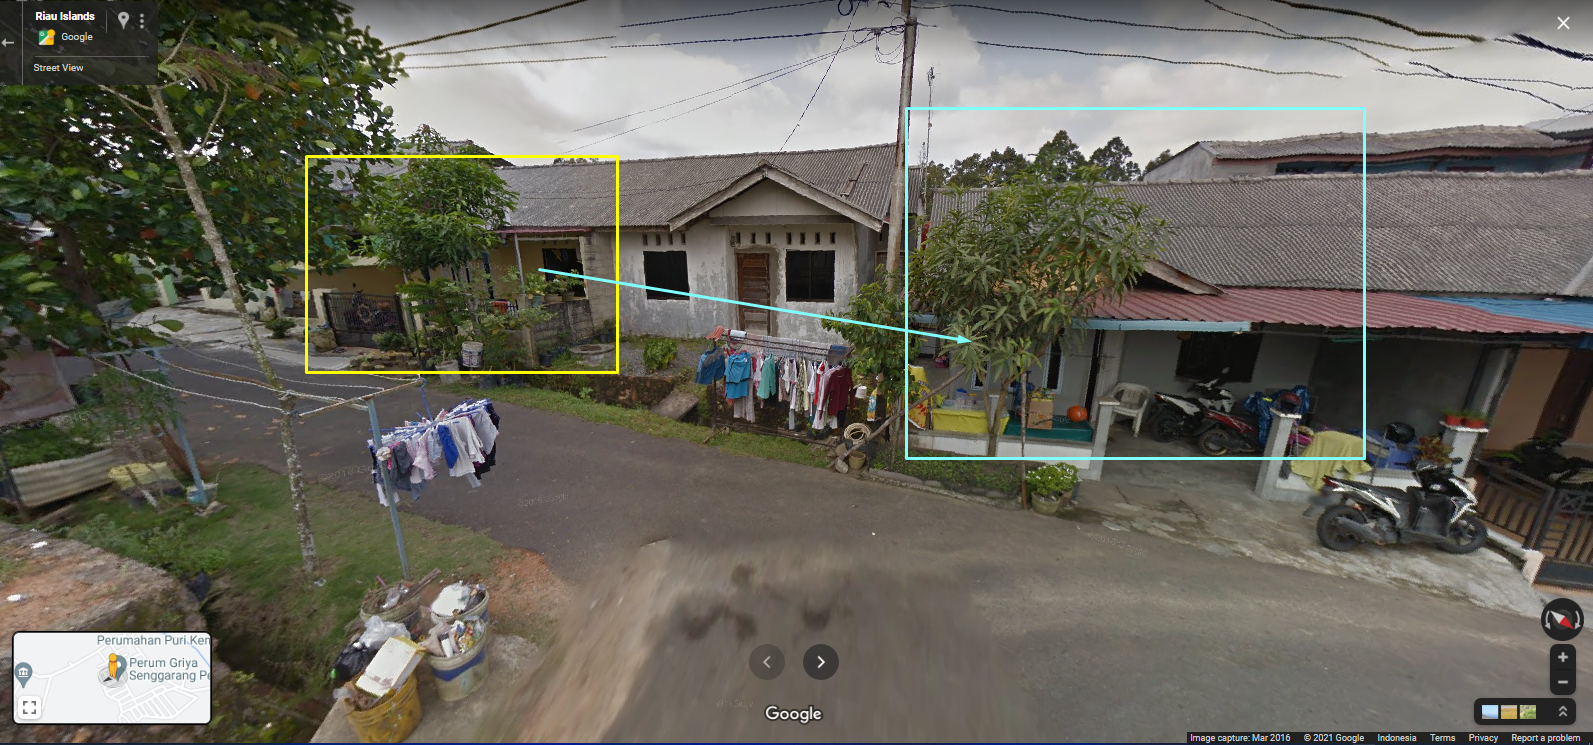
\includegraphics[width=0.5\textwidth]{gambar-lokasi.png}
    \caption{Location Measurements}
\end{figure}

in the picture above measured using a meter the distance is 8.5 meters with the router position in the house
This condition has obstacles because there are several walls that the signal must penetrate. so that what is obtained on the TL-WN722N receiver is not stable.

\begin{figure}[h]
    \centering
    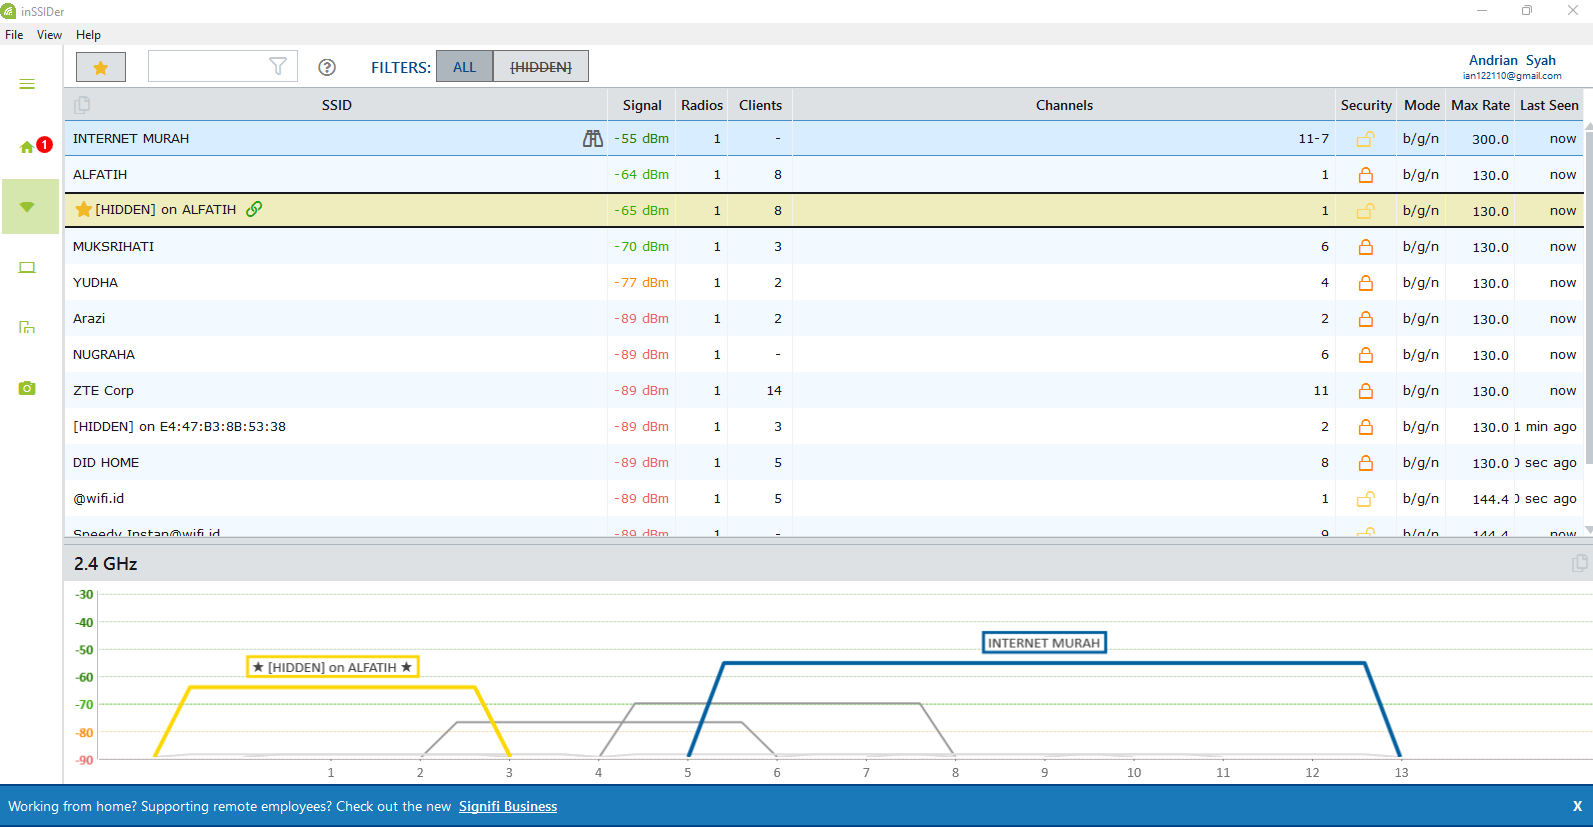
\includegraphics[width=0.5\textwidth]{gambar-inssider.png}
    \caption{Analize InSSIDer}
\end{figure}

we get a signal called "ALFATIH" of -65dBm in the HIDDEN position, if we look at HIDDEN this means that there is an SSID that is enabled for broadcast or broadcast.

\begin{figure}[h]
    \centering
    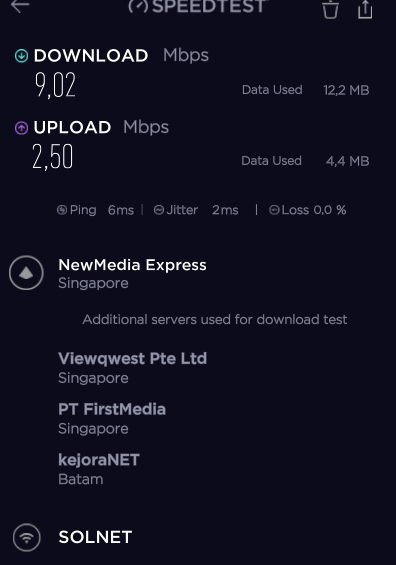
\includegraphics[width=0.4\textwidth]{speedtest.png}
    \caption{SpeedTest}
\end{figure}


In this test, the obstacle that exists between the receiver and the router is a wall that is only in the bulkhead. we can see that the speed we get from the ISP should be 1:2 with a 25 Mbps package.

\begin{figure}[h]
    \centering
    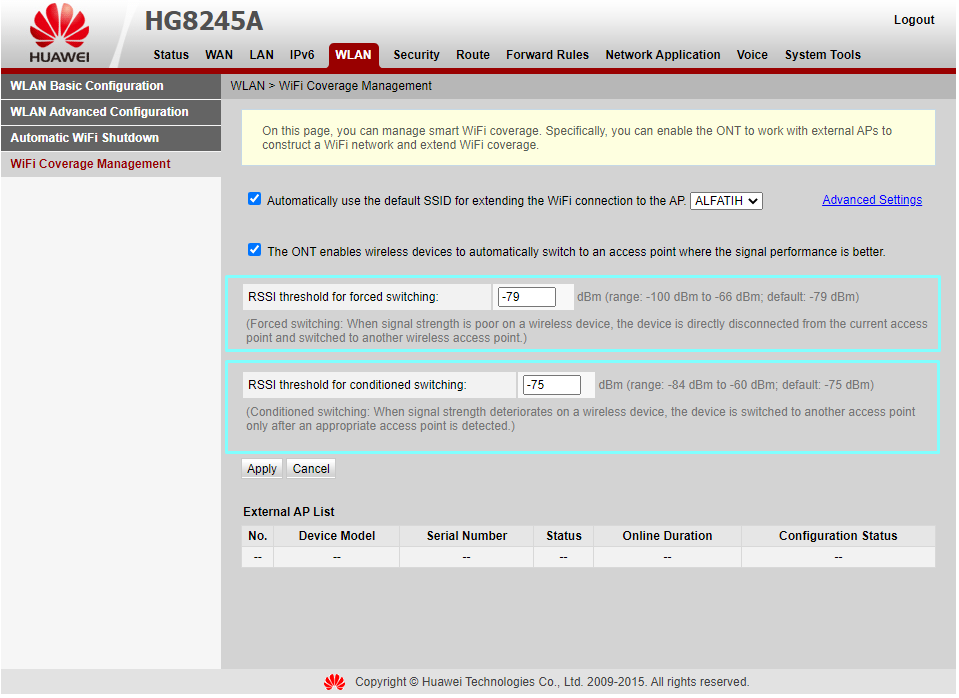
\includegraphics[width=0.5\textwidth]{router.png}
    \caption{Admin Page From Router Huawei HG8245}
\end{figure}


\begin{figure}[h]
    \centering
    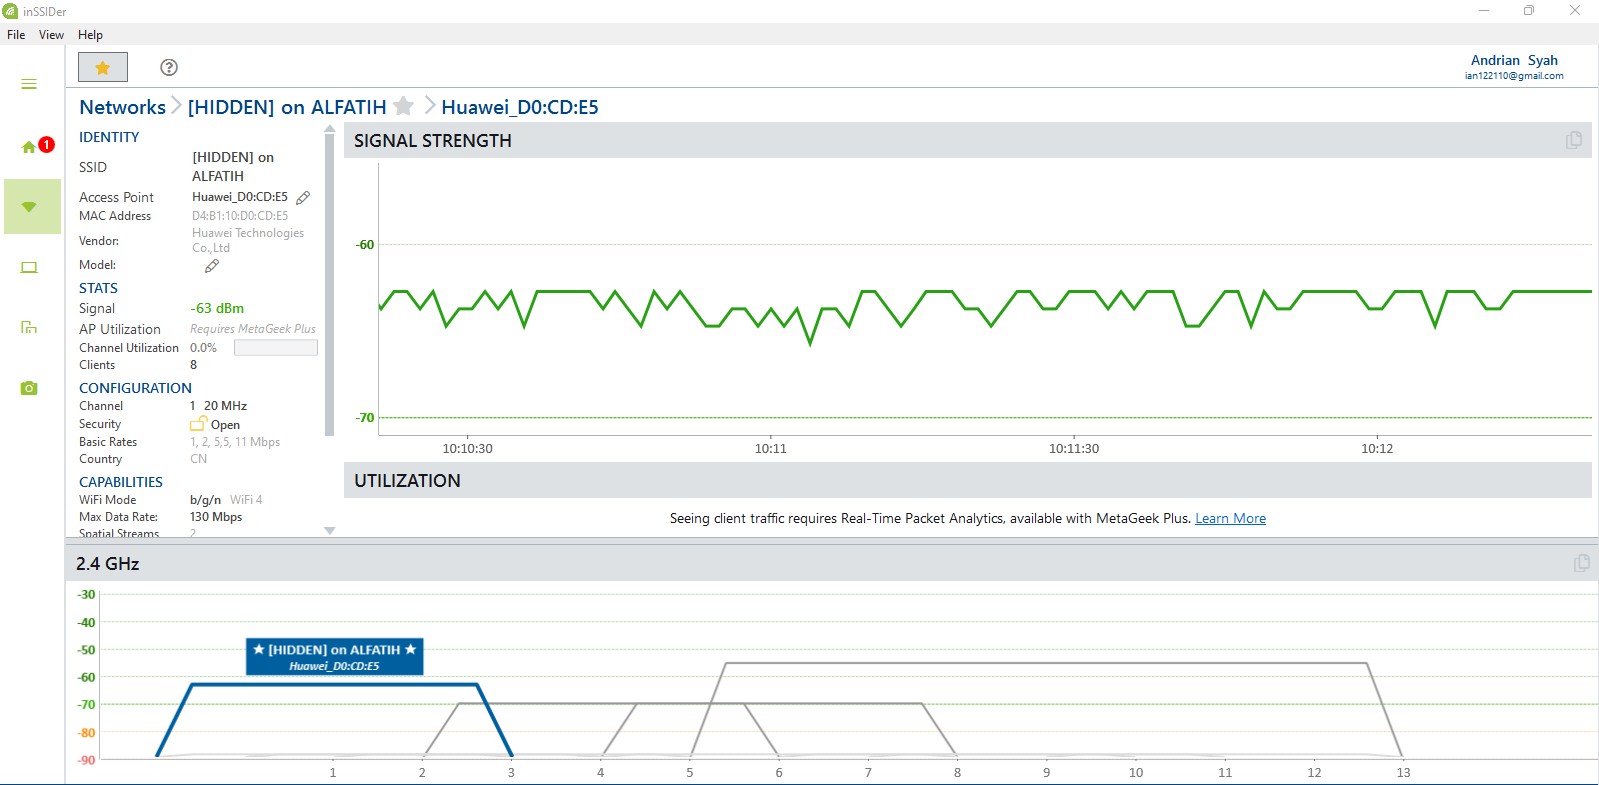
\includegraphics[width=0.5\textwidth]{signal-strengh.png}
    \caption{ Signal Strength View  }
\end{figure}

RSSI signal strength received by
receiver does not depend on distance
between transmitter and receiver, however
shows that there are large variations in fading
and shadowing at a location. This matter
seen at the measurement place that is in good condition
The environment has many properties such as
in the room there are partitions, walls, tables and
other properties, so that signal attenuation, signal deflection and reflection will occur
signal resulting in a strong drop
the signal emitted by the transmitter to the
receiver, even though the distance between the transmitter and
receiver close enough, but blocked by
there is a property around it, then strength
the signal will decrease and possibly
the signal strength will be equal to the strength
signal at the distance between transmitter and receiver
which is far enough away, but does not have
barrier around it. 

\section{Results and Discussion}

From the results of the wireless network analysis carried out in a residential environment between houses using a wireless usb signal receiver TP-LINK TL-WN722N, that is, when we walk to the 2nd floor in the Iteba campus area, the network will move
to the nearest access point with a double SSID thereby reducing transmission on a router, this is because the use of bands on the router is more than 1 SSID so
the resulting coverage is low and makes the accessed speed decrease when used in the SpeedTest By Ookla application~\cite{Ookla}.

\begin{equation}
   Average RSSI = \frac{Total values RSSI}{Total Coordinates receiver}
    \label{rerata_rssi}
\end{equation}

\begin{table}[htbp]
    \caption{Table Analize Measurements RSSI}
    \begin{center}
    \begin{tabular}{|c|c|c|c|}
        \hline
    \textbf{No} & \textbf{\textit{Tall}}& \textbf{\textit{Receiver}}& \textbf{\textit{Receiver signal average}} \\
    \hline
    1 & 178cm& 8 Receiver & -53.87 dbm  \\
    \hline
    2 & 180cm& 7 Receiver & -51.98 dbm  \\
    \hline
    \multicolumn{4}{l}{$^{\mathrm{a}}$Proceeds from InSSIDer funds}
    \end{tabular}
    \label{tab2}
    \end{center}
    \end{table}

\section{Conclusion}

A network will be inhibited if there is a wall and a wall that causes results
unstable and makes data transmission to the receiver device less and as a result buffering occurs, therefore there must be a repeater at every point
to ensure maximum data reception strength and no distortion of a wireless signal.

The use of the 2.4 GHz and 5 GHz bands actually doesn't affect it, but when we tested it when using the SSID Hotspot using the 5 Ghz band it wasn't detected on the laptop.
old or outdated, but on laptops that already support the 5 Ghz feature, you will be able to see the SSID that was created. ~\cite{weaver2013guide}

\begin{figure}[h]
    \centering
    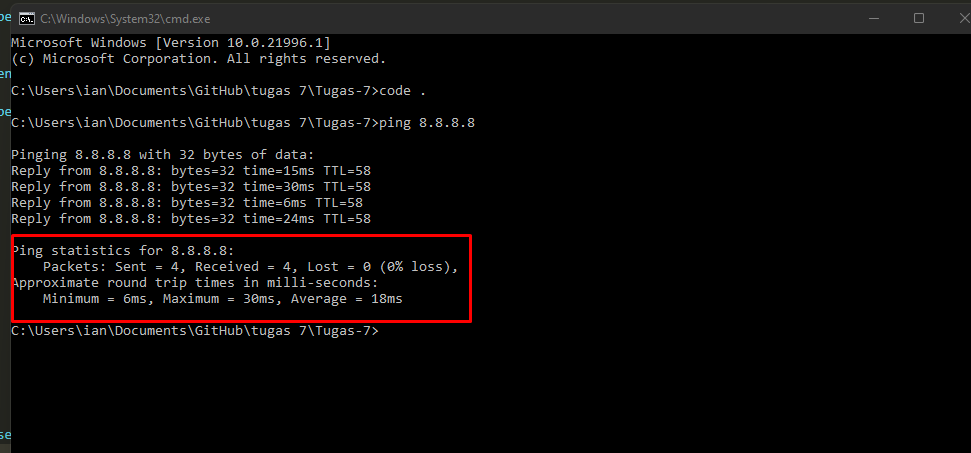
\includegraphics[width=0.5\textwidth]{ping.png}
    \caption{Measurements With Commad Promp}
\end{figure}

\bibliographystyle{IEEEtran}
\bibliography{referensi.bib}

\end{document}